\documentclass[twoside,a5paper,9pt]{extarticle}
%%%%%%%%%%%%%%%%%%%%%%%%%%%%%%%%%%%%%%%%%%%%%%%%%%%%%%%%%% 
% Autor: Alvaro Chirino, Fundación Aru 
% Versión: Noviembre, 2024
%%%%%%%%%%%%%%%%%%%%%%%%%%%%%%%%%%%%%%%%%%%%%%%%%%%%%%%%% 
%%% librerías base
%%%%%%%%%%%%%%%%%%%%%%%%%%%%%%%%%%%%%%%%%%%%%%%%%%%%%%%%% 
\usepackage[english,spanish]{babel}
\usepackage{booktabs}
\usepackage[utf8]{inputenc}
\usepackage[margin=0.6in,headheight=1pt]{geometry}
\usepackage{graphicx}
\usepackage[defaultfam,tabular,lining,extralight]{montserrat}
\usepackage{apacite}
\usepackage{natbib}
\usepackage{fancyhdr}
\pagestyle{fancy}
\fancyhead[RO,LE]{{\ifodd\value{page}\else\scriptsize\thetitle\fi}}
\fancyhead[RE,LO]{{\ifodd\value{page}\scriptsize\theauthor\else\fi}}
\renewcommand{\headrulewidth}{0pt}
\usepackage{titling}
\usepackage{hyperref}
\usepackage{float}
\usepackage{fontawesome}
%%%%%%%%%%%%%%%%%%%%%%%%%%%%%%%%%%%%%%%%%%%%%%%%%%%%%%%%%%%%%%%%%%%%%%%%%%%%%%%%%%%%
% (Opcional) Directorio para las figuras. Útil si se diferencia entre figuras con color (revista digital) y en blanco y negro (para impresión)
\graphicspath{{_fig_col/}}
%%%%%%%%%%%%%%%%%%%%%%%%%%%%%%%%%%%%%%%%%%%%%%%%%%%%%%%%%%%%%%%%%%%%%%%%%%%%%%%%%%%%
%%%%%%%%%%%%%%%%%%%%%%%%%%%%%%%%%%%%%%%%%%%%%%%%%%%%%%%%% librerías adicionales acá

%%%%%%%%%%%%%%%%%%%%%%%%%%%%%%%%%%%%%%%%%%%%%%%%%%%%%%%%%%%%%%%%%%%%%%%%%%%%%%%%%%%%
\predate{}
\postdate{}
\renewcommand{\footnotesize}{\fontsize{6pt}{10pt}\selectfont}
\pretitle{\begin{flushleft}\Huge}
\posttitle{\par\end{flushleft}}
\preauthor{\begin{flushright}
\large \lineskip 0.5em%
\begin{tabular}[t]{r}}
\postauthor{\end{tabular}\par \end{flushright}}
\renewenvironment{abstract}
 {\noindent\textbf{\abstractname:}\vspace{0.4cm}}
 
%%%%%%%%%%%%%%%%%%%%%%%%%%%
%%INCLUYA SU TÍTULO ACÁ
%%%%%%%%%%%%%%%%%%%%%%%%%%%

\title{\textbf{Título:} del documento\thanks{El contenido del presente documento es de responsabillidad de los autores y no compromete la opinión de Fundación ARU.}}

%%%%%%%%%%%%%%%%%%%%%%%%%%%
%%INCLUYA LOS AUTORES ACÁ
%%%%%%%%%%%%%%%%%%%%%%%%%%%

\author{Autor 1\thanks{Agradecimientos a \ldots por su colaboración \ldots. Comentarios y sugerencias son bienvenidos a: \ldots @aru.org.bo} \and Autor 2\thanks{\ldots}}
\date{}
\fancypagestyle{firstpage}{%
\fancyhead[R]{\vspace{0.2cm}\scriptsize ARU SEARCH: Revista de Investigación Aplicada de Economía Social y Desarrollo Nro X - MES AÑO}
\fancyhead[L]{}
}
\begin{document}

\maketitle
\pagenumbering{gobble}
\thispagestyle{firstpage}
%%%%%%%%%%%%%%%%%%%%%%%%%%%
%%INCLUYA RESÚMEN, CLASIFICACIÓN JEL Y PALABRAS CLAVE EN ESPAÑOL ACÁ
%% https://en.wikipedia.org/wiki/JEL_classification_codes
%% https://www.zbw.eu/stw/version/latest/about
%% https://www.aeaweb.org/jel/guide/jel.php
%%%%%%%%%%%%%%%%%%%%%%%%%%%
\begin{abstract}

Su resumen acá

\end{abstract}

\vspace{0.4cm}
\noindent
\scalebox{0.8}{
\begin{tabular}{lp{10cm}}
\textbf{Clasificación JEL:} & código 1, código 2, código 3, \ldots .\\% (https://www.aeaweb.org/econlit/jelCodes.php?view=jel)
\textbf{Palabras clave}: & palabra 1, palabra 2, palabra 3, \ldots .\\
\textbf{Repositorio de investigación \faGithub:} &  \url{https://github.com/ARUFoundation/AruSearch}
\end{tabular}}

\newpage
\pagenumbering{arabic}
\thispagestyle{fancy}
%%%%%%%%%%%%%%%%%%%%%%%%%%%
%%INCLUYA RESÚMEN, CLASIFICACIÓN JEL Y PALABRAS CLAVE EN INGLES ACÁ
%%%%%%%%%%%%%%%%%%%%%%%%%%%
\selectlanguage{english}
\begin{abstract}

Here!

\end{abstract}

\vspace{0.4cm}
\noindent
\scalebox{0.8}{
\begin{tabular}{lp{10cm}}
\textbf{JEL Classification:} & code 1, code 2, code 3, \ldots .\\% (https://www.aeaweb.org/econlit/jelCodes.php?view=jel)
\textbf{Keywords}: & word 1, word 2, word 3, \ldots .\\
\textbf{Research repository \faGithub:} &  \url{https://github.com/ARUFoundation/AruSearch}
\end{tabular}}
\selectlanguage{spanish} 

%%%%%%%%%%%%%%%%%%%%%%%%%%%
%%% INCLUYA EL CONTENIDO DE SU DOCUMENTO DE INVESTIGACIÓN ACÁ
%%%%%%%%%%%%%%%%%%%%%%%%%%%

\section{Introducción}

El contenido acá \ldots, y una figura de ejemplo en \ref{f1}

\begin{figure}[H]
\center
\caption{Ejemplo de figura}
\begin{tabular}{l}
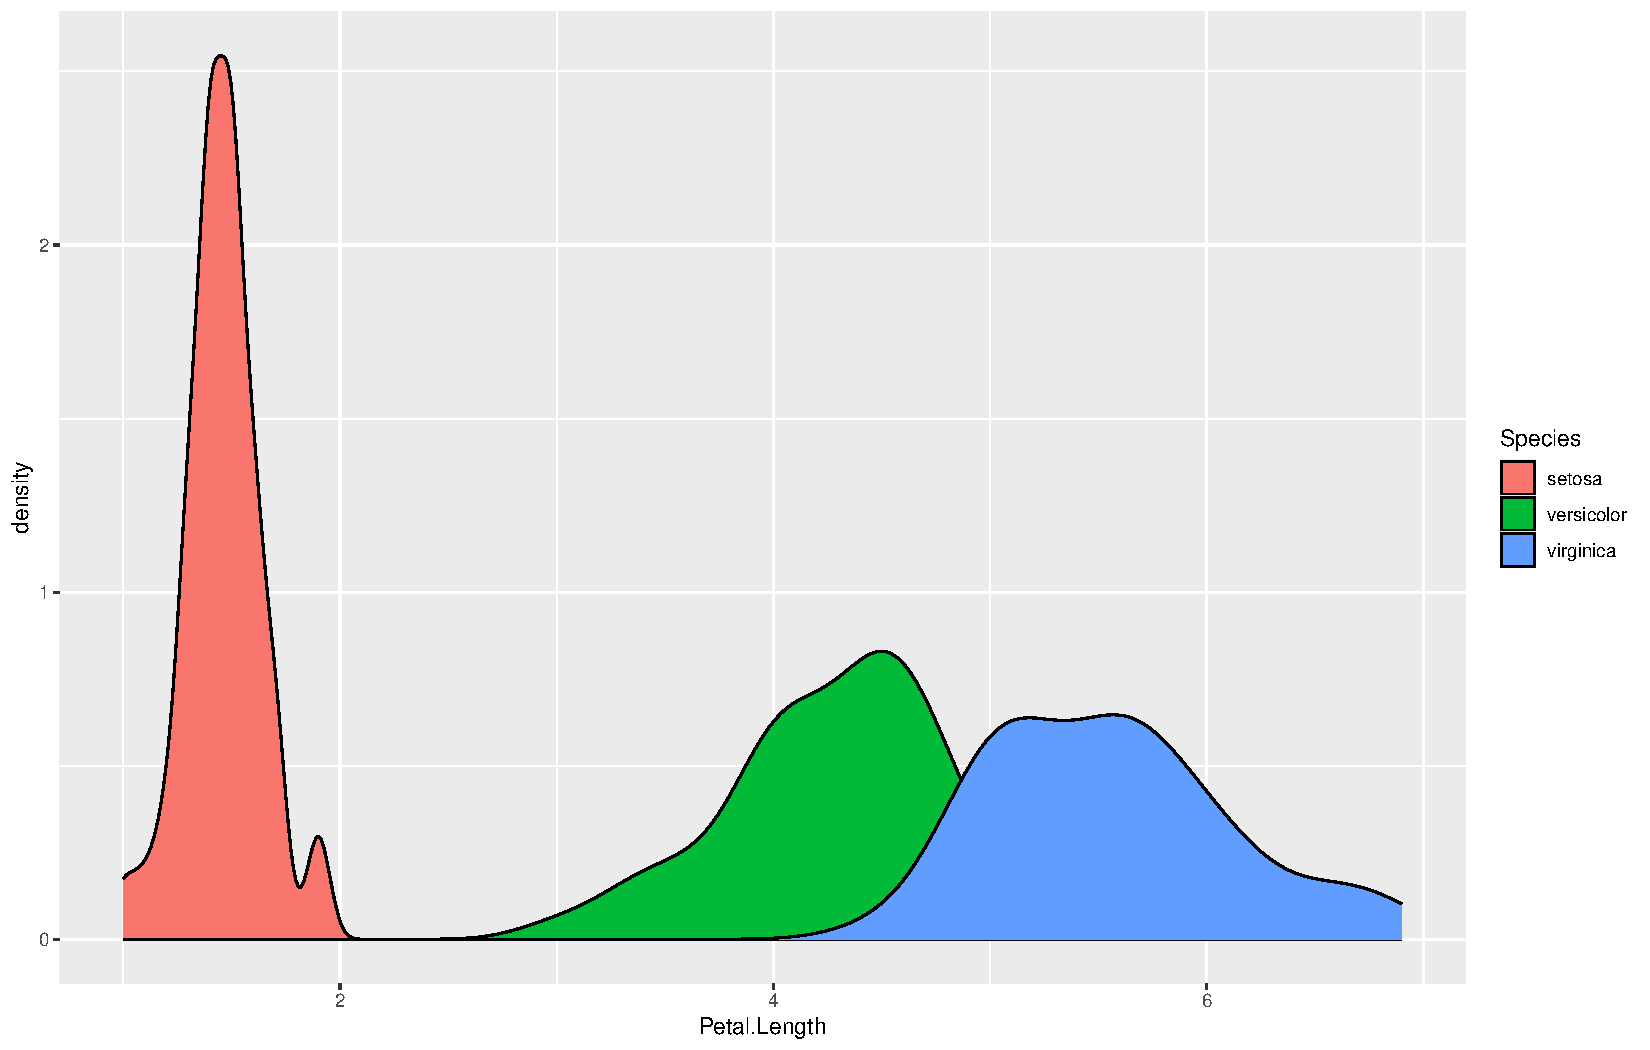
\includegraphics[scale=0.3]{example1}\\
\small{\textbf{Fuente:} \ldots}
\end{tabular}
\label{f1}	
\end{figure}

%%%%%%%%%%%%%%%%%%%%%%%%%%%
%%% INCLUYA EL NOMBRE DEL ARCHIVO .BIB "LAS REFERENCIAS DE SU DOCUMENTO" ACÁ:
%%% SE INCLUYE UN ARCHIVO DE REFERENCIA JUNTO A ESTA PLANTILLA. 
%%% https://www.bibtex.org/, SE RECOMIENDO EL USO DE ALGÚN GESTOR DE BIBLIOGRAFÍA PARA OPTIMIZAR ESTO; ZOTERO, MENDELEY, ENDNOTE
%%%%%%%%%%%%%%%%%%%%%%%%%%%
\bibliographystyle{apacite}
\bibliography{referencias}%Archivo .bib
\nocite*

% Anexos acá
\appendix

\end{document}
